
\chapter{Analysis and High-Level Design}

It is the goal of this thesis to enable detection of sleep-related illnesses 
with the aid of an Android device and low-cost sensors, and to further analyze 
and evaluate sleep- and breath-related patterns. We developed an application, 
called \textit{Nidra}, which attempts to collect, analyze and share data collected 
from external sensors, all on a mobile device. Also, Nidra acts as a platform for 
modules to enrich the data, thus extending the functionality of the application.

The motivation behind this application is to provide an interface for patients 
to potentially run a self-diagnostic (of the illness?) from home, and to aid 
researchers and doctors with analysis of sleep- and breathing-related illnesses 
(e.g., Obstructive Sleep Apnea). An overview of the Nidra application pipeline 
can be found in figure x, beginning with data acquired from a sensor, and ending 
with the data in the Nidra application. As for now, Nidra consists of three 
main functionalities, each related to the requirements defined in Section [Problem Statement]. 

\begin{enumerate}
    \item The application should provide an interface for the patient to 1) record physiological signals (i.e., during sleep); 2) present the results; and 3) export/import the results.
    \item The application should provide an interface for the developers to create modules to enrich the data from records or extend the functionality of the application. 
    \item The application should ensure a seamless and continuous data stream, uninterrupted from sensor disconnections and human disruptions.
\end{enumerate}

This chapter will give a detailed look at the design of Nidra...

\section{High-Level Design}

\subsection{Stakeholders}
A stakeholder is a term coined to describe those persons or organizations that have, or claim an interest in the project [Stakeholder defined, p. 4].  Identifying stakeholders is essential to fulfilling the requirement set in the thesis, as they contribute to form and sculpture the application. From the article [stakeholder defined, p.14] we can distinguish stakeholders into four categories: 1) \textit{contributing (primary) stakeholders} are those that participate in developing and sustaining the project; 2) \textit{observer (secondary) stakeholder} are those who affect or influence the project;  3) \textit{end-user (tertiary stakeholder)} is the one who interact and uses the output of the application; and 4) \textit{invested stakeholder} is one who has control of the project  [stakeholder defined, p. 13]. In Nidra, we have three stakeholders who affect the application, and each can be categorized respectfully.
\begin{itemize}
    \item \textbf{Patients} - are identified as an end-user; they interact with the application.  
    \item \textbf{Researchers/Doctors} - are identified as an observer stakeholder; they might not use the application itself. However, they might use the data obtained from the patients' recordings for further analysis. Additionally, request functionality in the application.
    \item \textbf{Developers} - are identified as a contributor stakeholder; they maintain the application from bugs or extend the functionally of the application. Additionally, they can contribute to developing modules that extend the functionality of the application. 
\end{itemize}


\subsection{Task Analysis}
Task analysis is a methodology to facilitate the design of complex systems. Hierarchical task analysis (HTA) is an underlying technique that analyzes and decomposes complex tasks such as planning, diagnosis, and decision making, into specific subtasks [Task analysis...]. In this Section, we will be analyzing system tasks and user-related tasks.

\subsubsection{System Tasks}

\textbf{Recording}

\noindent A \textit{recording} is a process of collecting and storing physiological signals from sensors over an extended period (i.e., overnight). To enable a recording, we need to establish connections to available sensors, collecting samples from the sensors and storing the samples on the device. A \textit{sensor} is a device that transforms analog signals from the real world into digital signals.  physiological signals over a medium (e.g., Bluetooth). The application and the sensors are separate components, and the communication between these components occurs over an application programming interface (API) [write more?]. A \textit{sample} is a single sensor reading containing data and metadata, such as time and physiological data.  
    
There are several approaches to assemble components to achieve a recording, and we review an alternative structure. In Figure \ref{fig:hta_recording} we have an HTA graph, which illustrate the building blocks to enable a recording and their dependencies:

\begin{figure}
    \centering
    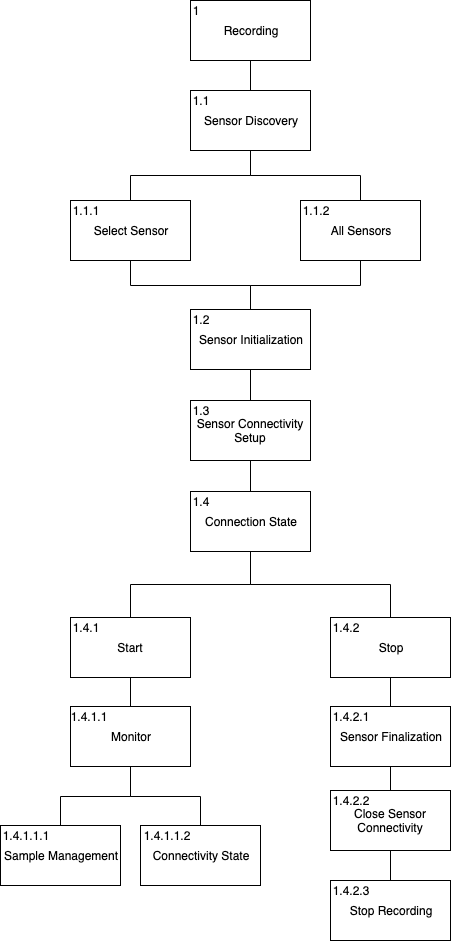
\includegraphics[width=0.65\textwidth]{images/Recording.png}
    \caption{Recording}
    \label{fig:hta_recording}
\end{figure}

\begin{itemize}
    \item Sensor Discover: Has to find all eligible sensors that can enable a recording.
    \item Select Sensors: From the sensor discovery, we can choose preferable sensors sources.
    \item  All Sensors: More straightforward, we sample from all of the available sensors.
    \item Sensor Initialization: Once we have a list of sensors sources, we need to establish and initialize a connection with the sensors. Occasionally a sensor might use some time to connect, or unforeseen occurrence is hindering the initialization of the sensor. Thus, blocking the state of the recording. 
    \item Sensor Connectivity Setup: Additionally, we establish a connection between the application and the sensor source. All data exchange occurs over the established interface. 
    \item Connection Stat: Based on sensors establishments we can proceed to either start or stop a recording. 
    \item Start: By starting, we notify the sensors to begin collecting data, and the view should display that a recording has begun accordingly.
    \item Monitor: Is continuously waiting for new samples to arrive on the interface defined between the application and the sensors.
    \item Sample Management: Once a new sample has arrived, we need to store the sample on a persistent storage.
    \item Connectivity State: If it is an external sensor, the sensor source might disconnect during a recording. Thus, implementing a mechanism to check for continuous data stream is a critical task.
    \item Stop: By stopping, we notify the sensors to stop collecting data from the sensor source.
    \item Sensor Finalization: We notify the sensor to stop sampling data, and close establishment.
    \item Close Sensor Connectivity: We close the interface establishment between the application and the sensors. 
    \item Stop Recording: Once the sensors has closed its connections, we can add additional information to the recording (e.g., title, description, rating). In the end, the recording has concluded and its stored on the mobile device.

\end{itemize}

This suggested structure of a recording is one alternative to enable a recording. Most of the components suggested in the structure are essential to a recording. A naive solution would be to ignore the connectivity state component, by assuming the sensors are connected indefinitely. In our thesis, we will be following 

\noindent \textbf{Sharing}

\noindent Sharing is a mechanism to export and import recordings across applications. \textit{Exporting} consists of bundling records with correlated samples into a format that can be transmitted. The format can be structured varyingly, however, we will discuss as few distinguishable formats that are applicable:

\begin{itemize}
    \item JSON - is a file format used to transmit data objects consisting of attribute-value pairs and array data types [wikipedia, JSON, 9.mai]. JSON has a simple syntax, which results in a compact file and efficient transmission. However, it only supports a few data types.
    \item XML - is a markup language that encodes arbitrary data structures into a format that is human-readable and machine-readable [wikipedia, XML, 9.mai]. XML provides a generalized markup that has support for numerous data types, structure validation, and extensions. However, the structure of XML results in a larger file[?]
    \item Constructing a file format solely for transmitting records and samples - by introducing a file format that is restrictive to the purpose of records and sample, we can minimize the transmitting file size. However, this might result in unreadable text, the overhead of parsing and transforming, and incompatibilities amongst devices. 
\end{itemize}
While these format structures are applicable for transmitting data, choosing a format that is compact, human-readable, and universal is essential. 

Once a preferred format for the recording is selected and stored in an exportable file, transferring the file to another device is made possible. One way is by transferring the files with the desired recipient through a server/middleware[?]; this makes it easier for users to share files amongst each other. Another way of transferring a file from one device to another is by sharing it through applicable mediums (e.g., email). The former requires additional functionality, such as registering users to distinguish recipients and additional security measurements for securing personal information. Therefore, a more preferable and secure solution would be to use the former solution. 

\textit{Importing} is accomplishable by locating the file, parsing the file, and storing the recordings in storage. A naive solution for the location of a file is by assuming that the file is located in on the same location amongst all devices, thus trying locating the file on a static location. Therefore, providing an interface to the users to deliberately locate the desired file in the file hierarchy of its device is practical. Android provides an interface for such a solution [?]. With the exact path of the file, we can read the bitstream of the file and parse the data according to the chosen format, and store the content of the file on the device.

\noindent \textbf{Modules}

\noindent Modules are independent applications that can be launched in the application to provide extended functionality and data enrichment. A module does not necessarily interact with the application itself. However, it utilizes the data (e.g., recordings) provided from the application. For instance, a module could be using the recordings to feed a machine learning algorithm to predict obstructive sleep apnea. Installing a module can be done by locating the module-application on the device, and can then be launched from the application. However, due to limitations in Android, the module-application cannot be executed within the application. Therefore, modules are run as independent application alongside the application.

The data exchange between a module and the application is possible on two various methods. One way is by selecting one or all of the recordings and bundling the data and sending it on launch. Another way is by establishing a direct communication link for pull-based requests, where the records are sent based on the requests of the module. The latter solution provides less overhead on data transfer; however, requires extended functionality to made possible. The former solution sends all of the selected data to the module on the launch, and there are no methods of communication with the application once a module is running. Essentially, the recordings do not change once it is on the device. Thus the former solution is feasible. 